\documentclass[12pt, a4paper, oneside]{ctexart}
\usepackage{amsmath, amsthm, amssymb, bm, graphicx, hyperref, geometry, mathrsfs,color}

\title{\huge\textbf{集合与实数集}}
\author{luojunxun}
\date{\today}
\linespread{2}%行间距
\geometry{left=2cm,right=2cm,top=2cm,bottom=2cm}%设置页面
\CTEXsetup[format={\Large\bfseries}]{section}%section左对齐


%定义环境
\newenvironment{Def}[1][def-name]{\par\noindent{\textit{(#1):}\small}}{\\\par}
\newenvironment{theorem}[1][Theorem-name]{\par\noindent \textbf{Theorem #1:}\textit}{\\\par}
\newenvironment{lemma}[1][lemma-name]{\par\noindent \textbf{Lemma #1:}\textbf}{\\\par}
\renewenvironment{proof}{\par\noindent{\textit{Proof:}\small}}{\\\par}
\newenvironment{example}[1][example-name]{\par{\textbf{Example:}}}{\\\par}
\newenvironment{say}{\center{\textit{summary:}}}{\\\par}
\newenvironment{note}[1][note-name]{\par\textit{#1:}}{\\\par}


\begin{document}
\maketitle

\section*{集合}
\Def[集族]{$\mathcal{X}=\{A\subset X\}$}:即$X$的某些子集构成的集合
\Def[幂集]{$\mathcal{P}(X)=\{X$的所有子集构成的集合$\}$}
\Def[集族的并]{$\bigcup A=\bigcup\limits_{\lambda\in\Lambda}A_\lambda=\{x|\exists A\subset X ;s.t. x\in A\}$}
\Def[集族的交]{$\bigcap A=\bigcap\limits_{\lambda\in\Lambda}A_\lambda=\{x|\forall A\subset X ; x\in A\}$}\\
这里的$\Lambda$是指标集,可以是有限集也可以是无限集

\section*{性质}
\theorem[集合运算的性质]{
    1.集合自己是自己的子集$\quad$2.集合的包含关系具有传递性$\quad$3.集合的取交取并运算有交换律,结合律,分配律$\quad$
    4.并集的补等于补集的交;交集的补等于补集的并
}

\Def[De-Moagan公式]{
    $(\bigcup\limits_{\lambda\in\Lambda}A_\lambda)^c=\bigcap\limits_{\lambda\in\Lambda}A_\lambda^c;
    (\bigcap\limits_{\lambda\in\Lambda}A_\lambda)^c=\bigcup\limits_{\lambda\in\Lambda}A_\lambda^c$
    }

\Def[对称差]{$A\Delta B=(A-B)\cup (B-A)=A\cup B-A\cap B$} 满足交换律
\Def[直积]{$X_1\times X_2=\{(x_1,x_2)|x_1\in X_1,x_2\in X_2\}$
    称为$X_1$和$X_2$的直积\\
    同样可以定义n维直积(或者可数多直积)$\prod\limits_{k=1}^nX_i$
}\\
在无穷维直积$\prod\limits_{k=1}^\infty X_i$中定义内积$<x,y>=\sum\limits_{i=1}^\infty x_iy_i$\\
定义度量(p范数)$||x||_p=(\sum\limits_{i=1}^\infty x_i^p)^{\frac{1}{p}}<+\infty;p\geq 1$\\
    这时候构成的空间我们称为巴拿赫空间$(l^p)(p\geq 1)$(无穷维)\\
    特别的:当$p=2$时,我们称其为希尔伯特空间(无穷维)$(l^2)$\\
    
    在n维希尔伯特空间(也就是欧几里得空间)中的范数为$Euclid$范数,且有如下性质\\
    1.非负性$d(x,y)\geq 0$当且仅当$x=y$取等\\
    2.对称性$d(x,y)=d(y,x)$\\
    3.三角不等式$d(x,y)\leq d(x,z)+d(y,z)\\\quad$
    事实上所有良定义的度量都要满足这三条性质
    
\note[赋范空间的构成]{$x\in l^p\iff \sum\limits_{i=1}^nx_i^p$收敛}
\example{$x=(\frac{1}{1^{\frac{3}{4}}},\frac{1}{2^{\frac{3}{4}}},\cdots,\frac{1}{n^{\frac{3}{4}}},\cdots)$}不属于$l^1$但是属于$l^2$
\\
\\

\section*{集合序列的极限}

\Def[集合序列]{$\{A_n\}_{n=1}^\infty=\{A_1,A_2,\cdots,A_n,\cdots\}$\\
若有$A_1\subset A_2\subset\cdots\subset A_n\subset \cdots$称序列$\{A_n\}_{n=1}^\infty$单增\\
若有$A_1\supset A_2\supset\cdots\supset A_n\supset \cdots$称序列$\{A_n\}_{n=1}^\infty$单减}

\Def[上下极限]{\\
    $B_n=\bigcup\limits_{k=n}^\infty A_n$;称$\{B_n\}_{n=1}^\infty$的交是序列$\{A_n\}_{n=1}^\infty$的上极限,记作
    $\varlimsup\limits_{n\to\infty}A_n=\bigcap\limits_{n=1}^\infty\bigcup\limits_{k\geq n}A_k$\\
    $C_n=\bigcap\limits_{k=n}^\infty A_n$;称$\{C_n\}_{n=1}^\infty$的并是序列$\{A_n\}_{n=1}^\infty$的下极限,记作
    $\varliminf\limits_{n\to\infty}A_n=\bigcup\limits_{n=1}^\infty\bigcap\limits_{k\geq n}A_k$\\
}
\note[性质]{\\
    1.$x\in \varlimsup\limits_{n\to\infty}A_n\iff \forall N,\exists n>N,s.t.x\in A_n \iff \{A_n\}_{n=1}^\infty$中有无穷多项包含$x$\\
    (就是说任何大的N后都有包含x的集合,但是这并不说明此后的集合都包含x,从而也可以有无穷多项集合不包含x)\\
    2.$x\in \varliminf\limits_{n\to\infty}A_n\iff \exists N_x,s.t.\forall n>N_x,x\in A_n\iff \{A_n\}_{n=1}^\infty$中只有有限多项不包含$x$\\
    (就是说有一个N可以控制x,使得从此以后的项都包含x,那么前面只有有限项不包含x)\\
    3.$\varliminf\limits_{n\to\infty}A_n\subset \varlimsup\limits_{n\to\infty}A_n$(即下极限包含在上极限中)\\
    4.当且仅当上极限等于下极限的时候称$\{A_n\}_{n=1}^\infty$的极限存在,记为$\lim\limits_{n\to\infty} A_n$\\
    5.当$A_n$单调的时候$\{A_n\}$一定有极限,此时(分别为单调增和单调减;${\color{red}这和数列极限不同,数列极限要单调有界才能说有极限,但是集合序列只需要单调}$)
    \[\lim\limits_{n\to\infty}A_n=\begin{cases}
        \bigcup\limits_{n=1}^\infty A_n\\
        \bigcap\limits_{n=1}^\infty A_n
    \end{cases}\]
    }
\begin{proof}[$A_n$单调]\\
    1.$A_n$增:$\varlimsup\limits_{n\to\infty}A_n=\bigcap\limits_{n=1}^\infty\bigcup\limits_{k\geq n}A_k=
    \bigcap\limits_{n=1}^\infty\bigcup\limits_{k=1}^\infty A_k=\bigcup\limits_{n=1}^\infty A_n$\\
    $\varliminf\limits_{n\to\infty}A_n=\bigcup\limits_{n=1}^\infty\bigcap\limits_{k\geq n}A_k=\bigcup\limits_{n=1}^\infty A_n$\\
    故上极限等于下极限等于$\bigcup\limits_{n=1}^\infty A_n$\\
    2.$A_n$减:$\varlimsup\limits_{n\to\infty}A_n=\bigcap\limits_{n=1}^\infty A_n$\\
    $\varliminf\limits_{n\to\infty}A_n=\bigcup\limits_{n=1}^\infty\bigcap\limits_{k\geq n}A_k=
    \bigcup\limits_{n=1}^\infty\bigcap\limits_{k=1}A_k=\bigcap\limits_{n=1}^\infty A_n$\\
    故上极限等于下极限等于$\bigcap\limits_{n=1}^\infty A_n$
\end{proof}

\Def[集合序列极限的相关性质]{
    \\
    {\color{red}1.$\bigcap\limits_{n=1}^\infty A_n \subset \varliminf\limits_{n\to\infty}A_n=\bigcup\limits_{n=1}^\infty\bigcap\limits_{k\geq n}A_k
    \subset \varlimsup\limits_{n\to\infty}A_n=\bigcap\limits_{n=1}^\infty\bigcup\limits_{k\geq n}A_k\subset \bigcup\limits_{n=1}^\infty A_n$}\\
    2.$(\varliminf\limits_{n\to\infty}A_n)^c=\varlimsup\limits_{n\to\infty}(A_n)^c\quad 
        (\varlimsup\limits_{n\to\infty}A_n)^c=\varliminf\limits_{n\to\infty}(A_n)^c$\\证明用德摩根律配合上下极限的定义就行
}




\example{例题1\\
    \begin{figure}[t]
        \begin{center}
        \centerline{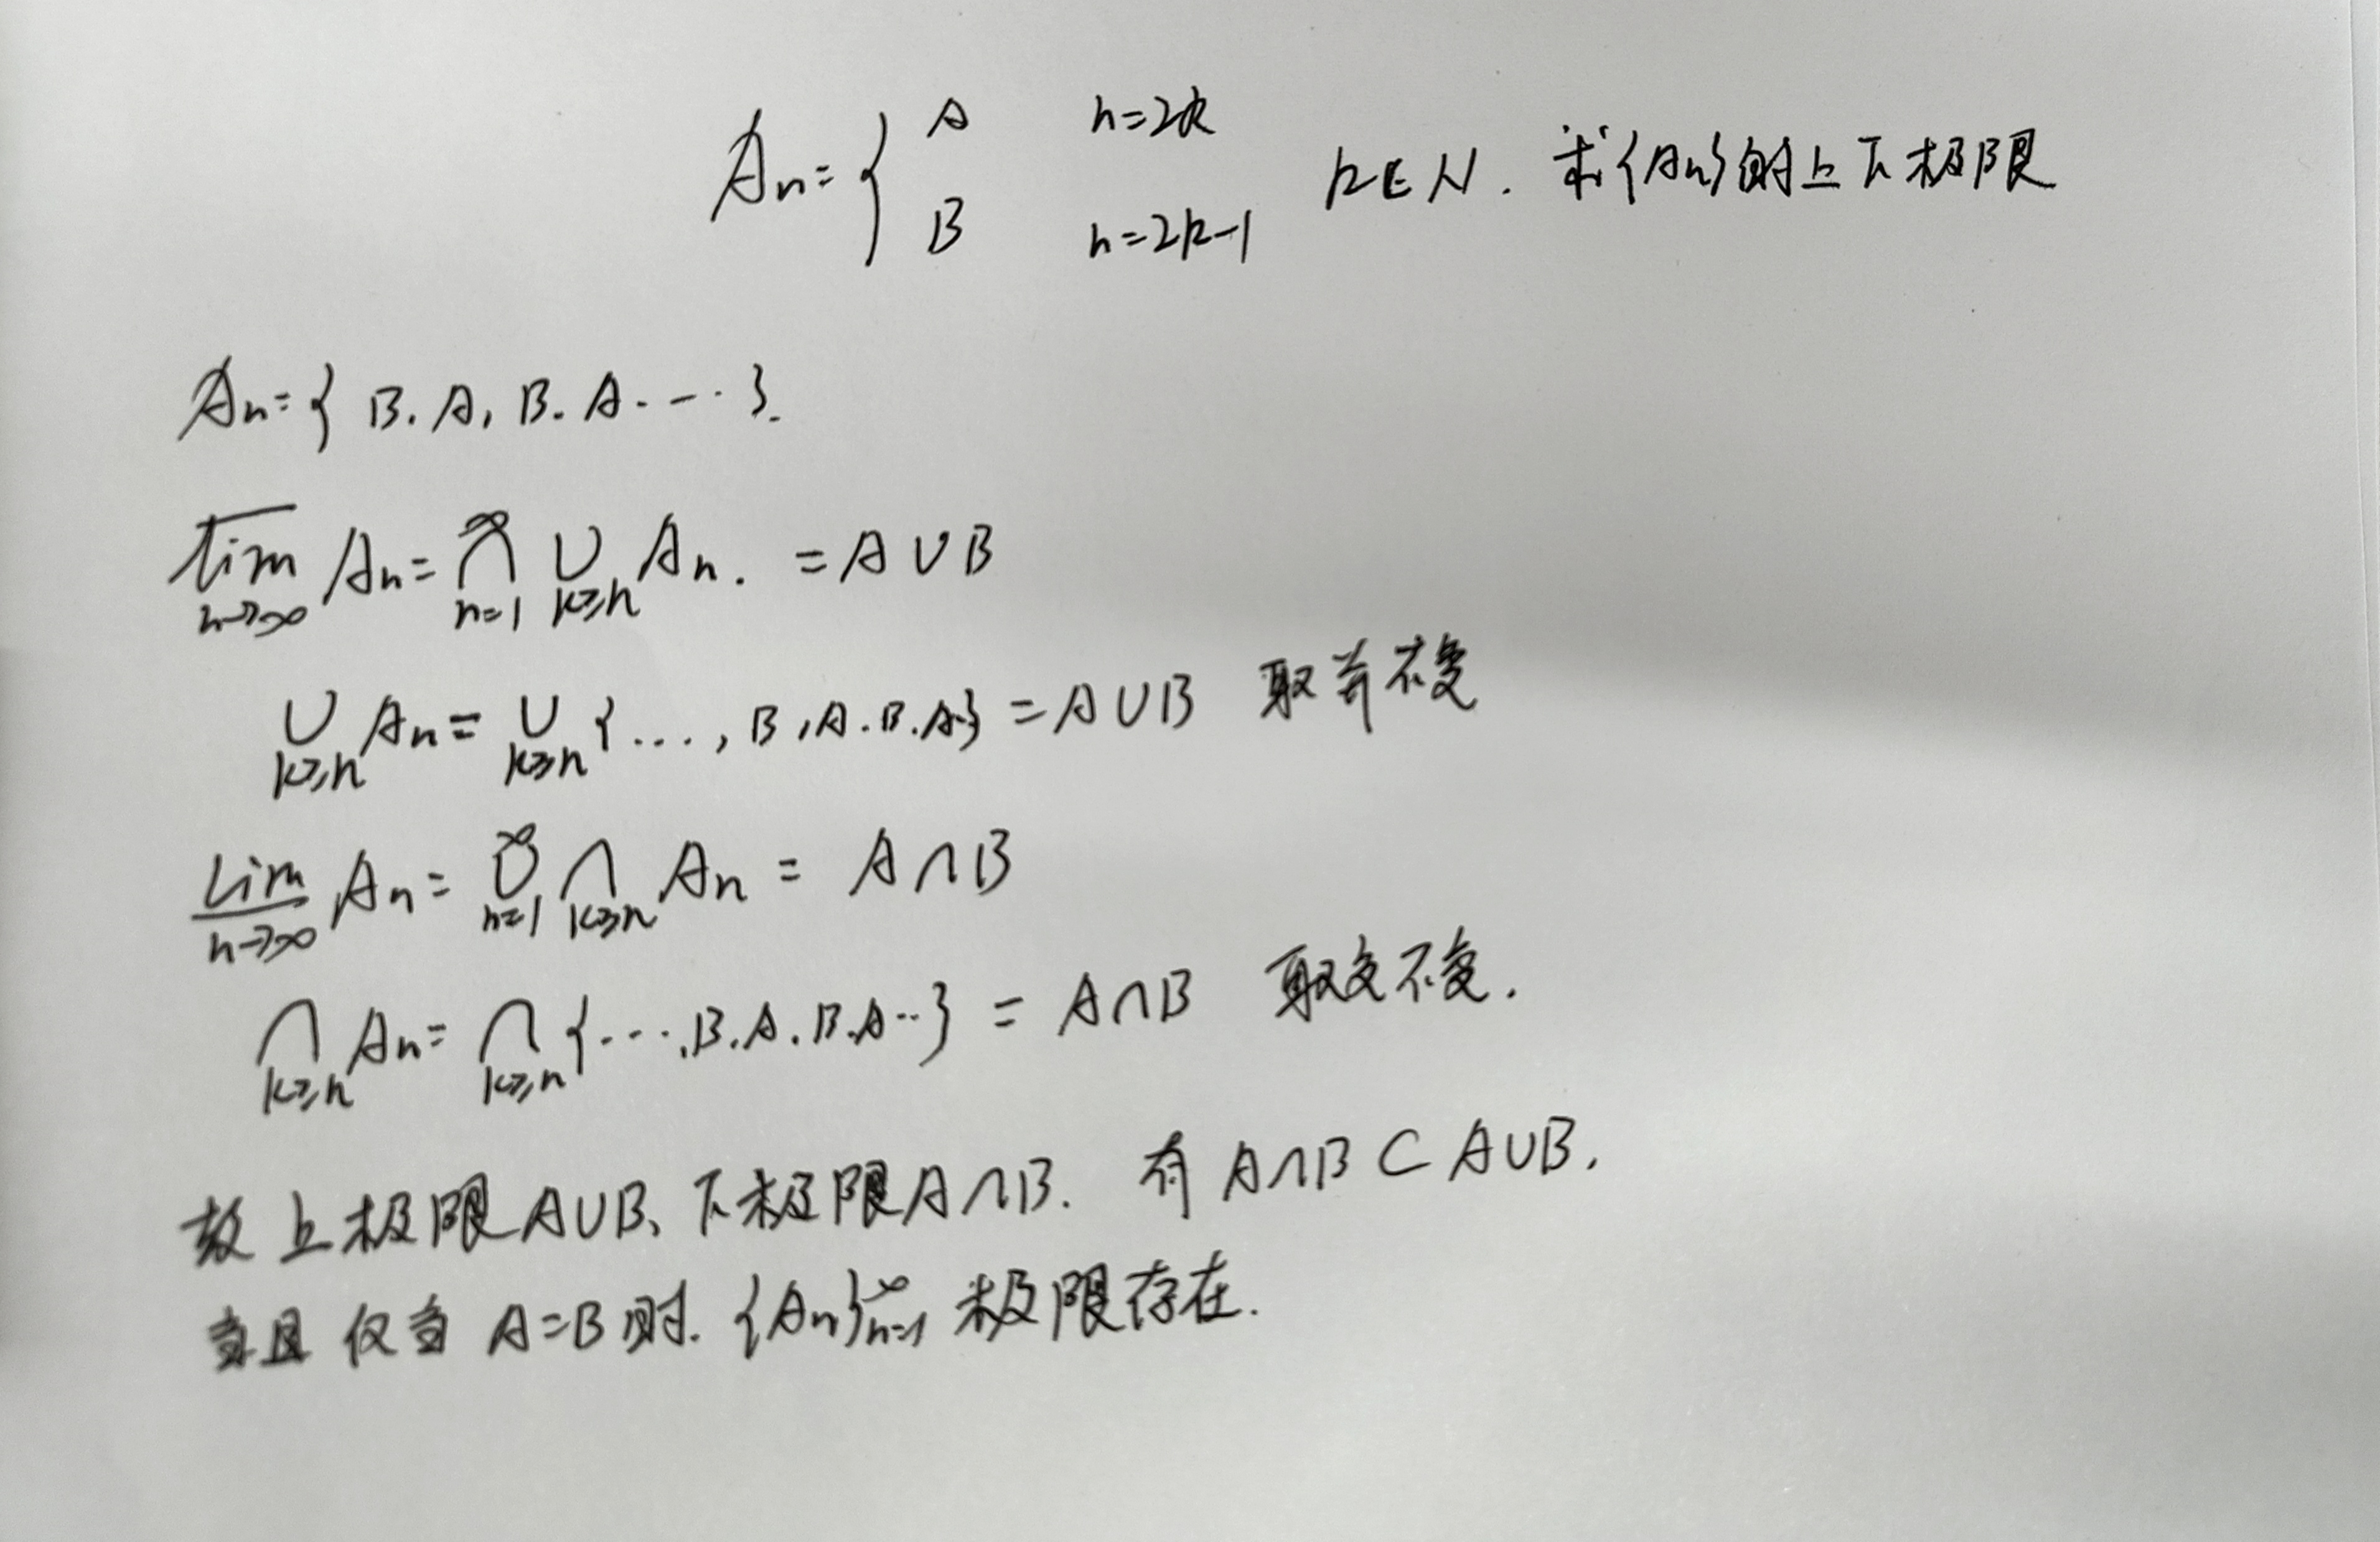
\includegraphics[scale=0.12]{example1.jpg}}
        \caption{一个求极限的例题}
        \label{figure}
        \end{center}
    \end{figure}

    \begin{figure}[p]

        \centerline{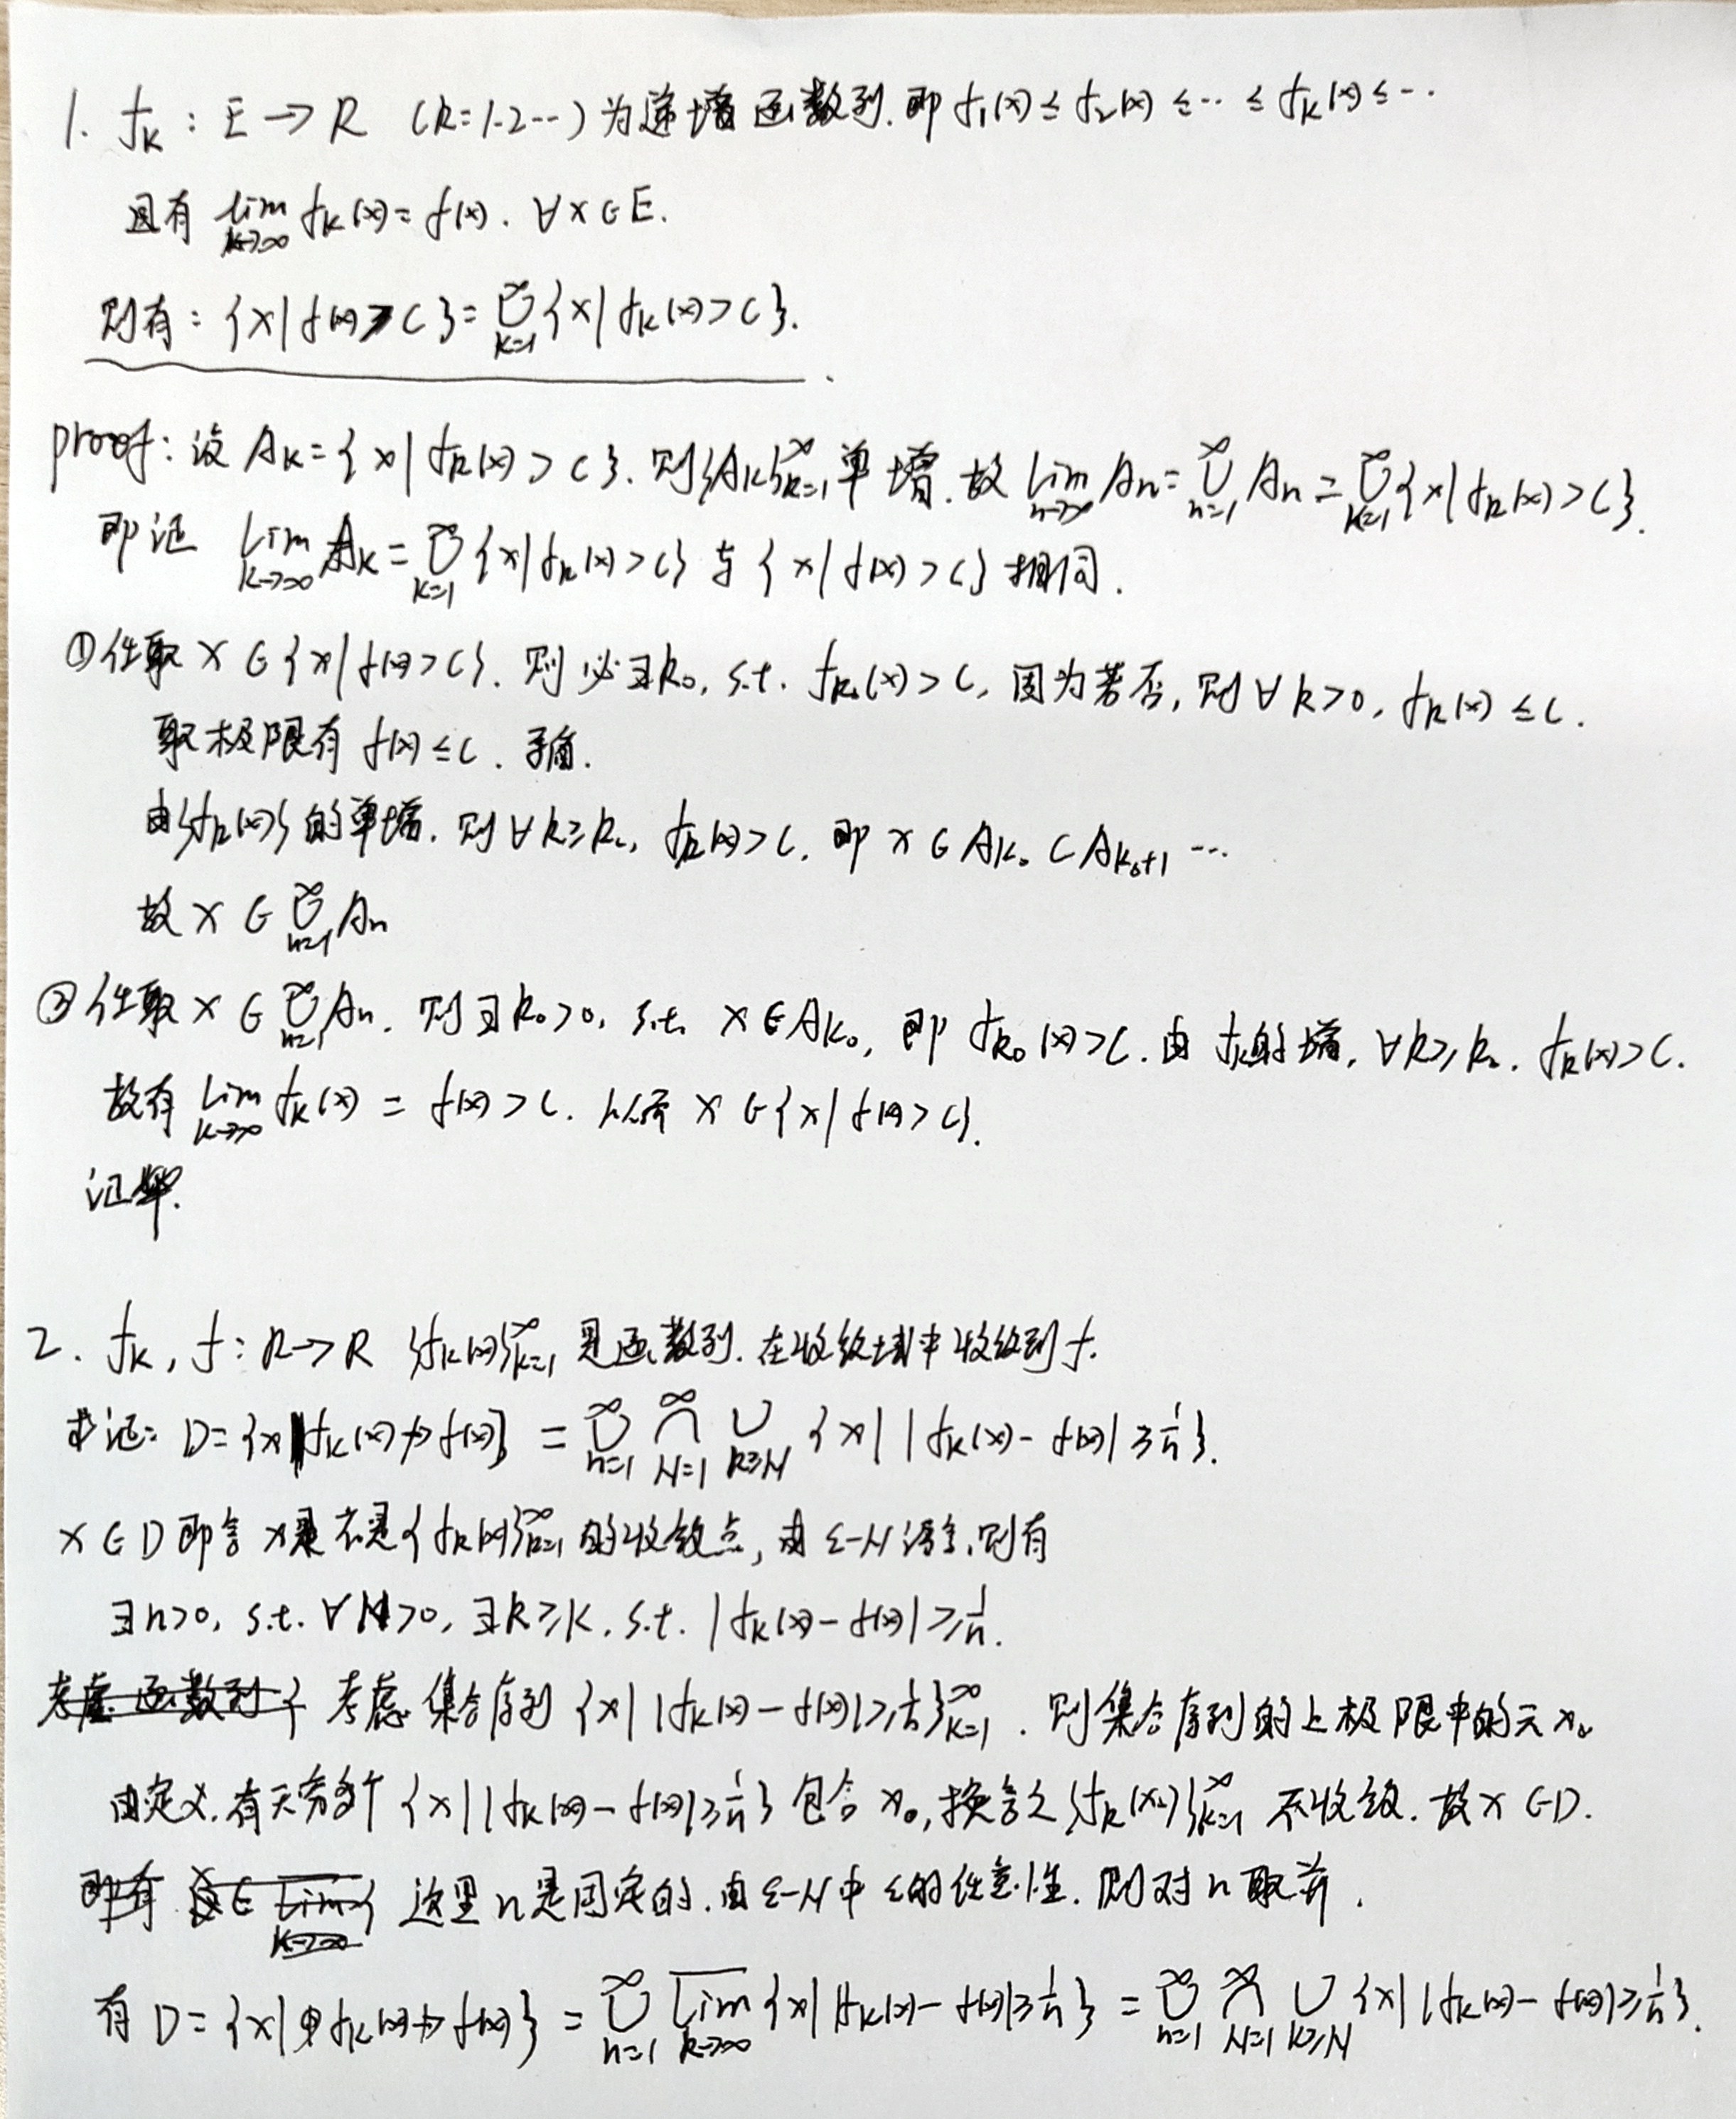
\includegraphics[width=1.2\linewidth,height=1.1\textheight]{example2.jpg}}
        \caption{课上习题}
        \label{figure}

    \end{figure}

       
}















\end{document}